\begin{titlepage} %% start document
	\centering %% bring everything in center of dokument
    
    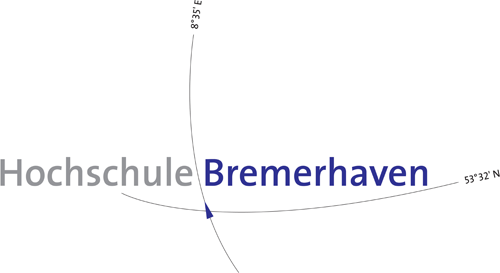
\includegraphics[scale = 0.4]{images/hs-logo.png}\\[1.5 cm]	%% quick way to include a graphic. DO NOT USE FOR FIGURES, SEE DOCUMENTATION HOW TO USE FIGURES 
    % Text in [] will give space between the lines
    \textsc{\LARGE University of Applied Sciences}\\[2.0 cm]%% University Name
	\textsc{\Large \sFaculty}\\[0.5 cm]				%% Course name
	\textsc{\large \sFirstTutor}\\[0.5 cm] %% Name of professor
    	
	\rule{\linewidth}{0.2 mm} \\[0.4 cm] %% create a line
	{ \huge \bfseries {\sTitle}}\\
	\rule{\linewidth}{0.2 mm} \\[1.5 cm] %% create a line
    %change here the distance when more than four authors
	
	\begin{minipage}{0.5\textwidth} %% create a table for authors and mat. numbers
		\begin{center} \large %% you can remove "\large" if many authors for more space
			\emph{Author:}\\
			\sName
			\end{center}
			\end{minipage}~
			\begin{minipage}{0.5\textwidth}
			\begin{center} \large %% you can remove "\large" if many authors for more space
			\emph{Mat. Number:} \\
            \sMtrNr								
		\end{center}
	\end{minipage}\\[1.5 cm] %% reduce here space between date to have it on titlepage when more than four authors
	
	{ \large Bremerhaven, the \today} %% show where and when (date)
    
%% end of document
\end{titlepage}